\documentclass[9pt]{IEEEtran}

\usepackage[english]{babel}
\usepackage{graphicx}
\usepackage{epstopdf}
\usepackage{fancyhdr}
\usepackage{amsmath}
\usepackage{amsthm}
\usepackage{amssymb}
\usepackage{url}
\usepackage{array}
\usepackage{textcomp}
\usepackage{listings}
\usepackage{hyperref}
\usepackage{xcolor}
\usepackage{colortbl}
\usepackage{float}
\usepackage{gensymb}
\usepackage{longtable}
\usepackage{supertabular}
\usepackage{multicol}

\usepackage[utf8x]{inputenc}

\usepackage[T1]{fontenc}
\usepackage{lmodern}{}
\input{glyphtounicode}
\pdfgentounicode=1

\graphicspath{{./figures/}}
\DeclareGraphicsExtensions{.pdf,.png,.jpg,.eps}

% correct bad hyphenation here
\hyphenation{op-tical net-works semi-conduc-tor trig-gs}

% ============================================================================================

\title{\vspace{0ex}
Artificial Neural Networks}

\author{Marko Medved\vspace{-4.0ex}}

% ============================================================================================

\begin{document}

\maketitle

\section{Implementation of fully connected neural network for classification}
\subsection{Implementation details}
We implemented a fully connected neural network with an arbitrary number of layers for
 a classification task. We applied the sigmoid activation function at each layer, except
  for the input and output layers. Since the task involves multi-class classification,
   we used the softmax function on the output layer (applied to the logits).

To train the network, we used an approach where gradients are computed 
separately for each training example and then accumulated. We used the 
cross-entropy loss (log loss) as the criterion. After computing the loss,
 we applied backpropagation to calculate the gradients and then performed 
 standard gradient descent to update the model parameters. 

 To correctly perform backpropagation, the following gradients were calculated. 
 First, the gradient of the loss function with respect to the logits was computed. 
 This was done by combining the gradient of the loss with respect to the probabilities 
 and the gradient of the probabilities with respect to the logits (i.e., the gradient of the softmax):
\[
\frac{\partial L}{\partial z_j} =
\begin{cases}
p_j - 1 & \text{if } j = y_i \\
p_j & \text{otherwise}
\end{cases}
\]
where $y_i$ is the true class, $z_j$ are the logits and $p_j$ are the probabilities of 
each class. 

Next, the gradients for the weights and biases in the linear layer were calculated:
\[
\frac{\partial L}{\partial \mathbf{W}^{(k)}} = \delta^{(k)} \cdot \left( \mathbf{a}^{(k-1)} \right)^T
\quad \text{and} \quad
\frac{\partial L}{\partial \mathbf{b}^{(k)}} = \delta^{(k)}
\]
where $ \delta^{(k)}$ is the gradient of the  pre-activations in the current layer and $a^{k-1}$ is the 
vector of activations in the previous layer. 

Lastly, we needed to compute the gradient of the activations and consequently the pre-activations 
(note that in this case, \(k\) refers to the next layer, so it corresponds to \(k-1\) in the
 previous equation):

\[
\sigma'(z^{(k)}) = \sigma(z^{(k)}) \cdot \left(1 - \sigma(z^{(k)})\right)
\]
\[
\delta^{(k)} = \left( \delta^{(k+1)} \cdot \mathbf{W}^{(k+1)} \right) \circ \sigma'(z^{(k)})
\]
where \( \sigma(z^{(k)}) \) represents the sigmoid function applied to the pre-activations.

\subsection{Comparison of gradients to numerical gradients}
To validate our implementation of backpropagation, we added the option to return both 
the numerical gradients and the gradients computed through backpropagation at a chosen
 layer. Our comparison procedure involved computing the gradients for all samples in the 
 dataset (using the provided squares, doughnut, and example datasets), and then comparing 
 the results.

We used a network with six hidden layers, each with a different number of 
activations. We then checked the differences between the
 numerical and backpropagation-based gradients for both weights
  and biases. In all cases, the differences were within acceptable
   bounds—none of the gradient differences exceeded \(1 \times 10^{-7}\).

\subsection{Fitting the network to the squares and doughnut data}
Next, we fitted our implementation to the squares and doughnut datasets to 
demonstrate that the network is capable of fully learning non-linear patterns.

In Figure~\ref{fig:doughnut}, we observe that the network successfully fits the doughnut dataset. 
For this task, we used a network with a single hidden layer
 containing 3 activation units and a learning rate of 1.

\begin{figure}[h]
    \centering
    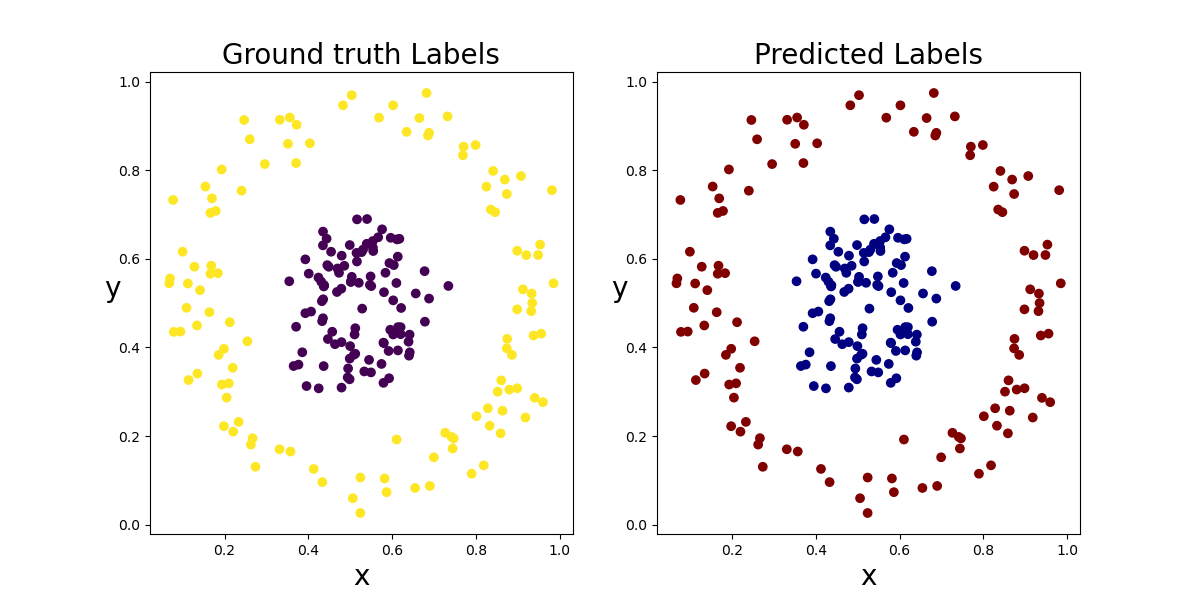
\includegraphics[width=1\columnwidth]{figures/doughnut.png}
    \caption{Network predictions fitted on the doughnut dataset.}
    \label{fig:doughnut}
\end{figure}

Similarly, in Figure~\ref{fig:squares}, the network also manages to perfectly fit the squares dataset. 
This time, we used one hidden layer with 5 activation units, keeping the learning rate at 1.

\begin{figure}[h]
    \centering
    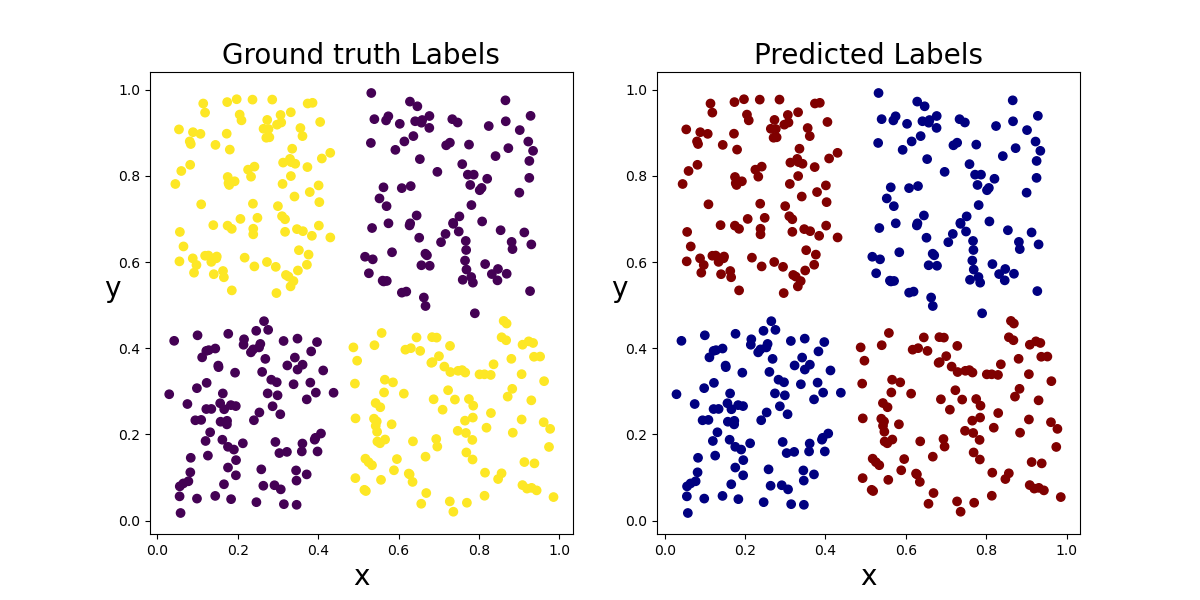
\includegraphics[width=1\columnwidth]{figures/squares.png}
    \caption{Network predictions fitted on the squares dataset.}
    \label{fig:squares}
\end{figure}

\section{Extending the ANN implementation}
\subsection{Adding support for regression}
We also implemented the regression counterpart of the same neural network.
 The key differences in implementation compared to the classification network are outlined below:

\begin{itemize}
    \item The final layer contains a single output unit instead of one per class.
    \item No softmax function is applied in the output layer.
    \item The loss function used is the mean squared error, based on the assumption of a normally distributed target variable.
    \item The only change in the backpropagation algorithm occurs in the final layer, where the gradient is scaled by a constant factor of 2 (in comparison to the classification network).
\end{itemize}

\subsection{Adding regularization}
We also added the support for L2 regularization for both classification and regression networks. 
Note that the regularization was only applied to the weights, not to the biases.
It was implemented by adding the correct term in gradient descent
  as shown by the following formula:

\[
\mathbf{W}^{(k)} \leftarrow \mathbf{W}^{(k)} - \eta \left( \nabla_{\mathbf{W}^{(k)}} L + 2\lambda \mathbf{W}^{(k)} \right)
\]

\subsection{Adding reLU support}
Next, we added support for the ReLU activation function. This required modifying the gradient computations, as the ReLU function and its derivative are defined as follows:
\[
\text{ReLU}(x) = \max(0, x)
\]
\[
\text{ReLU}'(x) =
\begin{cases}
1 & \text{if } x > 0 \\
0 & \text{otherwise}
\end{cases}
\]
Additionally, we allowed users to customize the activation function used at each layer of the network.

\subsection{Comparing our implementation with PyTorch}

\bibliographystyle{IEEEtran}
\bibliography{bibliography}

\end{document}
